

\tikzset{every picture/.style={line width=0.75pt}} %set default line width to 0.75pt        

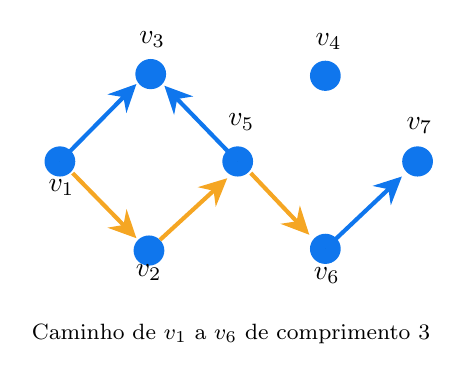
\begin{tikzpicture}[x=0.75pt,y=0.75pt,yscale=-1,xscale=1]
%uncomment if require: \path (0,175); %set diagram left start at 0, and has height of 175

%Shape: Ellipse [id:dp5077982020192706] 
\draw  [draw opacity=0][fill={rgb, 255:red, 15; green, 118; blue, 237 }  ,fill opacity=1 ] (17.01,71.75) .. controls (17.01,67.74) and (20.33,64.48) .. (24.42,64.48) .. controls (28.51,64.48) and (31.83,67.74) .. (31.83,71.75) .. controls (31.83,75.77) and (28.51,79.02) .. (24.42,79.02) .. controls (20.33,79.02) and (17.01,75.77) .. (17.01,71.75) -- cycle ;
%Shape: Ellipse [id:dp7144769570638401] 
\draw  [draw opacity=0][fill={rgb, 255:red, 15; green, 118; blue, 237 }  ,fill opacity=1 ] (59.92,114.67) .. controls (59.92,110.66) and (63.24,107.41) .. (67.33,107.41) .. controls (71.42,107.41) and (74.74,110.66) .. (74.74,114.67) .. controls (74.74,118.69) and (71.42,121.94) .. (67.33,121.94) .. controls (63.24,121.94) and (59.92,118.69) .. (59.92,114.67) -- cycle ;
%Shape: Ellipse [id:dp10535612642783376] 
\draw  [draw opacity=0][fill={rgb, 255:red, 15; green, 118; blue, 237 }  ,fill opacity=1 ] (60.76,29.66) .. controls (60.76,25.64) and (64.08,22.39) .. (68.17,22.39) .. controls (72.26,22.39) and (75.58,25.64) .. (75.58,29.66) .. controls (75.58,33.67) and (72.26,36.93) .. (68.17,36.93) .. controls (64.08,36.93) and (60.76,33.67) .. (60.76,29.66) -- cycle ;
%Shape: Ellipse [id:dp8289908753476658] 
\draw  [draw opacity=0][fill={rgb, 255:red, 15; green, 118; blue, 237 }  ,fill opacity=1 ] (102.67,71.75) .. controls (102.67,67.74) and (105.99,64.48) .. (110.08,64.48) .. controls (114.17,64.48) and (117.49,67.74) .. (117.49,71.75) .. controls (117.49,75.77) and (114.17,79.02) .. (110.08,79.02) .. controls (105.99,79.02) and (102.67,75.77) .. (102.67,71.75) -- cycle ;
%Shape: Ellipse [id:dp06972249328365487] 
\draw  [draw opacity=0][fill={rgb, 255:red, 15; green, 118; blue, 237 }  ,fill opacity=1 ] (144.9,113.85) .. controls (144.9,109.83) and (148.22,106.58) .. (152.31,106.58) .. controls (156.4,106.58) and (159.72,109.83) .. (159.72,113.85) .. controls (159.72,117.86) and (156.4,121.12) .. (152.31,121.12) .. controls (148.22,121.12) and (144.9,117.86) .. (144.9,113.85) -- cycle ;
%Shape: Ellipse [id:dp7147960092743524] 
\draw  [draw opacity=0][fill={rgb, 255:red, 15; green, 118; blue, 237 }  ,fill opacity=1 ] (189.33,71.75) .. controls (189.33,67.74) and (192.65,64.48) .. (196.74,64.48) .. controls (200.83,64.48) and (204.15,67.74) .. (204.15,71.75) .. controls (204.15,75.77) and (200.83,79.02) .. (196.74,79.02) .. controls (192.65,79.02) and (189.33,75.77) .. (189.33,71.75) -- cycle ;
%Shape: Ellipse [id:dp469938637266508] 
\draw  [draw opacity=0][fill={rgb, 255:red, 15; green, 118; blue, 237 }  ,fill opacity=1 ] (144.9,30.48) .. controls (144.9,26.47) and (148.22,23.21) .. (152.31,23.21) .. controls (156.4,23.21) and (159.72,26.47) .. (159.72,30.48) .. controls (159.72,34.5) and (156.4,37.75) .. (152.31,37.75) .. controls (148.22,37.75) and (144.9,34.5) .. (144.9,30.48) -- cycle ;
%Straight Lines [id:da4397858754948907] 
\draw [color={rgb, 255:red, 15; green, 118; blue, 237 }  ,draw opacity=1 ][fill={rgb, 255:red, 0; green, 0; blue, 0 }  ,fill opacity=1 ][line width=1.5]    (24.42,71.75) -- (58.47,37.29) ;
\draw [shift={(61.28,34.45)}, rotate = 494.65] [fill={rgb, 255:red, 15; green, 118; blue, 237 }  ,fill opacity=1 ][line width=0.08]  [draw opacity=0] (13.4,-6.43) -- (0,0) -- (13.4,6.44) -- (8.9,0) -- cycle    ;
%Straight Lines [id:da7612336938851023] 
\draw [color={rgb, 255:red, 15; green, 118; blue, 237 }  ,draw opacity=1 ][fill={rgb, 255:red, 0; green, 0; blue, 0 }  ,fill opacity=1 ][line width=1.5]    (110.08,71.75) -- (77.52,38.15) ;
\draw [shift={(74.74,35.27)}, rotate = 405.90999999999997] [fill={rgb, 255:red, 15; green, 118; blue, 237 }  ,fill opacity=1 ][line width=0.08]  [draw opacity=0] (13.4,-6.43) -- (0,0) -- (13.4,6.44) -- (8.9,0) -- cycle    ;
%Straight Lines [id:da521868726384179] 
\draw [color={rgb, 255:red, 245; green, 166; blue, 35 }  ,draw opacity=1 ][fill={rgb, 255:red, 0; green, 0; blue, 0 }  ,fill opacity=1 ][line width=1.5]    (30.56,77.37) -- (58.48,105.88) ;
\draw [shift={(61.28,108.73)}, rotate = 225.6] [fill={rgb, 255:red, 245; green, 166; blue, 35 }  ,fill opacity=1 ][line width=0.08]  [draw opacity=0] (13.4,-6.43) -- (0,0) -- (13.4,6.44) -- (8.9,0) -- cycle    ;
%Straight Lines [id:da3551036263203664] 
\draw [color={rgb, 255:red, 245; green, 166; blue, 35 }  ,draw opacity=1 ][fill={rgb, 255:red, 0; green, 0; blue, 0 }  ,fill opacity=1 ][line width=1.5]    (72.63,109.56) -- (102.08,82.55) ;
\draw [shift={(105.03,79.84)}, rotate = 497.48] [fill={rgb, 255:red, 245; green, 166; blue, 35 }  ,fill opacity=1 ][line width=0.08]  [draw opacity=0] (13.4,-6.43) -- (0,0) -- (13.4,6.44) -- (8.9,0) -- cycle    ;
%Straight Lines [id:da5375483437520805] 
\draw [color={rgb, 255:red, 245; green, 166; blue, 35 }  ,draw opacity=1 ][fill={rgb, 255:red, 0; green, 0; blue, 0 }  ,fill opacity=1 ][line width=1.5]    (116.38,77.37) -- (141.82,104.18) ;
\draw [shift={(144.57,107.08)}, rotate = 226.5] [fill={rgb, 255:red, 245; green, 166; blue, 35 }  ,fill opacity=1 ][line width=0.08]  [draw opacity=0] (13.4,-6.43) -- (0,0) -- (13.4,6.44) -- (8.9,0) -- cycle    ;
%Straight Lines [id:da8162139572767808] 
\draw [color={rgb, 255:red, 15; green, 118; blue, 237 }  ,draw opacity=1 ][fill={rgb, 255:red, 0; green, 0; blue, 0 }  ,fill opacity=1 ][line width=1.5]    (152.31,113.85) -- (186.26,81.77) ;
\draw [shift={(189.17,79.02)}, rotate = 496.62] [fill={rgb, 255:red, 15; green, 118; blue, 237 }  ,fill opacity=1 ][line width=0.08]  [draw opacity=0] (13.4,-6.43) -- (0,0) -- (13.4,6.44) -- (8.9,0) -- cycle    ;

% Text Node
\draw (17.43,78.78) node [anchor=north west][inner sep=0.75pt]    {$v_{1}$};
% Text Node
\draw (59.5,120.05) node [anchor=north west][inner sep=0.75pt]    {$v_{2}$};
% Text Node
\draw (61.18,7.8) node [anchor=north west][inner sep=0.75pt]    {$v_{3}$};
% Text Node
\draw (146.16,8.62) node [anchor=north west][inner sep=0.75pt]    {$v_{4}$};
% Text Node
\draw (104.09,47.42) node [anchor=north west][inner sep=0.75pt]    {$v_{5}$};
% Text Node
\draw (145.32,121.51) node [anchor=north west][inner sep=0.75pt]    {$v_{6}$};
% Text Node
\draw (189.91,49.07) node [anchor=north west][inner sep=0.75pt]    {$v_{7}$};
% Text Node
\draw (9.39,148.44) node [anchor=north west][inner sep=0.75pt]  [font=\footnotesize] [align=left] {Caminho de $\displaystyle v_{1}$ a $\displaystyle v_{6}$ de comprimento 3};


\end{tikzpicture}